\documentclass{beamer}
\usepackage[utf8]{inputenc}

\usetheme{Madrid}
\usecolortheme{default}
\usepackage{amsmath,amssymb,amsfonts,amsthm}
\usepackage{txfonts}
\usepackage{tkz-euclide}
\usepackage{listings}
\usepackage{adjustbox}
\usepackage{array}
\usepackage{tabularx}
\usepackage{gvv}
\usepackage{lmodern}
\usepackage{circuitikz}
\usepackage{tikz}
\usepackage{graphicx}

\setbeamertemplate{page number in head/foot}[totalframenumber]

\usepackage{tcolorbox}
\tcbuselibrary{minted,breakable,xparse,skins}



\definecolor{bg}{gray}{0.95}
\DeclareTCBListing{mintedbox}{O{}m!O{}}{%
	breakable=true,
	listing engine=minted,
	listing only,
	minted language=#2,
	minted style=default,
	minted options={%
		linenos,
		gobble=0,
		breaklines=true,
		breakafter=,,
		fontsize=\small,
		numbersep=8pt,
		#1},
	boxsep=0pt,
	left skip=0pt,
	right skip=0pt,
	left=25pt,
	right=0pt,
	top=3pt,
	bottom=3pt,
	arc=5pt,
	leftrule=0pt,
	rightrule=0pt,
	bottomrule=2pt,
	toprule=2pt,
	colback=bg,
	colframe=orange!70,
	enhanced,
	overlay={%
		\begin{tcbclipinterior}
			\fill[orange!20!white] (frame.south west) rectangle ([xshift=20pt]frame.north west);
	\end{tcbclipinterior}},
	#3,
}
\lstset{
	language=C,
	basicstyle=\ttfamily\small,
	keywordstyle=\color{blue},
	stringstyle=\color{orange},
	commentstyle=\color{green!60!black},
	numbers=left,
	numberstyle=\tiny\color{gray},
	breaklines=true,
	showstringspaces=false,
}
%------------------------------------------------------------
%This block of code defines the information to appear in the
%Title page
\title %optional
{2.4.33}
\date{}
%\subtitle{A short story}

\author % (optional)
{M Chanakya Srinivas- EE25BTECH11036}




\begin{document}


\frame{\titlepage}


%----------------- Problem -------------------
\begin{frame}{Problem}
Name the type of triangle formed by the points
\[
A(-5,6), \quad B(-4,-2), \quad C(7,5).
\]
\end{frame}

%----------------- Vertices -------------------
\begin{frame}{Vertices}
\begin{align}
\vec{A} &= \myvec{-5\\6}, \nonumber \\
\vec{B} &= \myvec{-4\\-2}, \nonumber \\
\vec{C} &= \myvec{7\\5} \label{eq:vertices}
\end{align}
\end{frame}

%----------------- Difference vectors -------------------
\begin{frame}{Difference Vectors}
\begin{align}
\vec{B}-\vec{A} &= \myvec{1\\-8}, \label{eq:BA} \\[4pt]
\vec{C}-\vec{A} &= \myvec{12\\-1}, \label{eq:CA} \\[4pt]
\vec{C}-\vec{B} &= \myvec{11\\7}. \label{eq:CB}
\end{align}
\end{frame}

%----------------- Angle at A -------------------
\begin{frame}{Angle at A}
\begin{align}
(\vec{B}-\vec{A})^\top(\vec{C}-\vec{A})
&= \myvec{1 & -8}\myvec{12\\-1} \nonumber \\
&= 12+8 = 20 > 0 \label{eq:dotA}
\end{align}
So, $\angle A$ is acute.
\end{frame}

%----------------- Angle at B -------------------
\begin{frame}{Angle at B}
\begin{align}
(\vec{A}-\vec{B})^\top(\vec{C}-\vec{B})
&= \myvec{-1 & 8}\myvec{11\\7} \nonumber \\
&= -11+56 = 45 > 0 \label{eq:dotB}
\end{align}
So, $\angle B$ is acute.
\end{frame}

%----------------- Angle at C -------------------
\begin{frame}{Angle at C}
\begin{align}
(\vec{A}-\vec{C})^\top(\vec{B}-\vec{C})
&= \myvec{-12 & 1}\myvec{-11\\-7} \nonumber \\
&= 132-7 = 125 > 0 \label{eq:dotC}
\end{align}
So, $\angle C$ is acute.
\end{frame}

%----------------- Conclusion -------------------
\begin{frame}{Conclusion}
All dot products are positive $\;\Rightarrow\;$ all angles are acute.  
Also, side lengths are unequal $\;\Rightarrow\;$ scalene.  

\[
\boxed{\text{The triangle is an acute scalene triangle.}}
\]
\end{frame}





% --- Frame 1: C Code ---
\begin{frame}[fragile]{C Code}
\begin{lstlisting}[language=C]
#include <stdio.h>
#include <math.h>

// Function to compute squared distance using matrices
double dist2(double P[2], double Q[2]) {
    double diff[2];
    diff[0] = P[0] - Q[0];
    diff[1] = P[1] - Q[1];
    return diff[0]*diff[0] + diff[1]*diff[1];
}

int main() {
    double A[2] = {-5, 6};
    double B[2] = {-4, -2};
    double C[2] = {7, 5};

    // Distances squared
    double AB2 = dist2(A, B);
    double BC2 = dist2(B, C);
    \end{lstlisting}
\end{frame}

    \begin{frame}[fragile]{C Code}
\begin{lstlisting}
    double CA2 = dist2(C, A);

    printf("AB^2 = %.2lf, BC^2 = %.2lf, CA^2 = %.2lf\n", AB2, BC2, CA2);

    // Check for type
    if (fabs(AB2 - BC2) < 1e-6 || fabs(BC2 - CA2) < 1e-6 || fabs(CA2 - AB2) < 1e-6)
        printf("The triangle is Isosceles.\n");
    else
        printf("The triangle is Scalene.\n");

    if (fabs(AB2 + BC2 - CA2) < 1e-6 || fabs(BC2 + CA2 - AB2) < 1e-6 || fabs(CA2 + AB2 - BC2) < 1e-6)
        printf("It is also a Right-angled triangle.\n");

    return 0;
}
\end{lstlisting}
\end{frame}

% --- Frame 2: Only Python Code ---
\begin{frame}[fragile]{Only Python Code}
\begin{lstlisting}[language=Python]
import sys
sys.path.insert(0, '/home/chanakya/MATGEO/2.4.33/codes')   # path to local scripts
import numpy as np
import numpy.linalg as LA
import matplotlib.pyplot as plt

# local imports
from libs.line.funcs import *

# Function to compute squared distance
def dist2(P, Q):
    return LA.norm(P-Q)**2

# Given points
A = np.array([-5, 6]).reshape(-1,1)
B = np.array([-4, -2]).reshape(-1,1)
C = np.array([7, 5]).reshape(-1,1)
\end{lstlisting}
\end{frame}
\begin{frame}[fragile]{Only Python Code}
\begin{lstlisting}
# Distances squared
AB2 = dist2(A,B)
BC2 = dist2(B,C)
CA2 = dist2(C,A)

# Determine type
triangle_type = []
if np.isclose(AB2, BC2) or np.isclose(BC2, CA2) or np.isclose(CA2, AB2):
    triangle_type.append("Isosceles")
else:
    triangle_type.append("Scalene")

if (np.isclose(AB2+BC2, CA2) or
    np.isclose(BC2+CA2, AB2) or
    np.isclose(CA2+AB2, BC2)):
    triangle_type.append("Right-angled")

triangle_type = " ".join(triangle_type)
\end{lstlisting}
\end{frame}
\begin{frame}[fragile]{Only Python Code}
\begin{lstlisting}
# Generate triangle sides
x_AB = line_gen(A,B)
x_BC = line_gen(B,C)
x_CA = line_gen(C,A)

# Plotting
plt.plot(x_AB[0,:], x_AB[1,:], label='$AB$')
plt.plot(x_BC[0,:], x_BC[1,:], label='$BC$')
plt.plot(x_CA[0,:], x_CA[1,:], label='$CA$')

# Labeling the coordinates
tri_coords = np.block([[A,B,C]])
vert_labels = ['A','B','C']
for i, txt in enumerate(vert_labels):
    plt.annotate(f'{txt}({int(tri_coords[0,i])},{int(tri_coords[1,i])})',
                 (tri_coords[0,i], tri_coords[1,i]),
                 textcoords="offset points",
                 xytext=(20,5), ha='center')
\end{lstlisting}
\end{frame}
\begin{frame}[fragile]{Only Python Code}
\begin{lstlisting}
# Show triangle type at centroid
centroid = (A+B+C)/3
plt.text(centroid[0,0], centroid[1,0],
         f"{triangle_type} Triangle",
         fontsize=12, color='green',
         bbox=dict(facecolor='yellow', alpha=0.3, edgecolor='black'))

# Axes formatting
ax = plt.gca()
ax.spines['top'].set_color('none')
ax.spines['right'].set_color('none')
ax.spines['left'].set_position('zero')
ax.spines['bottom'].set_position('zero')

plt.grid()
\end{lstlisting}
\end{frame}
\begin{frame}[fragile]{Only Python Code}
\begin{lstlisting}
plt.axis('equal')
plt.legend(loc='best')
plt.title("Triangle ABC with Classification")
plt.show()
\end{lstlisting}
\end{frame}

% --- Frame 3: Python Code with Shared Output ---
\begin{frame}[fragile]{Python Code with Shared Output}
\begin{lstlisting}[language=Python]
import numpy as np
import matplotlib.pyplot as plt

# Points (convert to numpy int to ensure matrix ops but cast for display)
A = np.array([-5, 6])
B = np.array([-4, -2])
C = np.array([7, 5])

# Matrix difference and squared distance
def dist2(P, Q):
    diff = P - Q
    return diff @ diff   # dot product

# Distances squared
AB2 = dist2(A, B)
BC2 = dist2(B, C)
CA2 = dist2(C, A)
\end{lstlisting}
\end{frame}
\begin{frame}[fragile]{Python Code with Shared Output}
\begin{lstlisting}
# Determine type
triangle_type = []
if np.isclose(AB2, BC2) or np.isclose(BC2, CA2) or np.isclose(CA2, AB2):
    triangle_type.append("Isosceles")
else:
    triangle_type.append("Scalene")

if (np.isclose(AB2 + BC2, CA2) or 
    np.isclose(BC2 + CA2, AB2) or 
    np.isclose(CA2 + AB2, BC2)):
    triangle_type.append("Right-angled")

triangle_type = " ".join(triangle_type)

print(f"AB^2 = {AB2}, BC^2 = {BC2}, CA^2 = {CA2}")
print(f"The triangle is {triangle_type}.")

# ---- Plotting ----
X = [A[0], B[0], C[0], A[0]]
Y = [A[1], B[1], C[1], A[1]]
\end{lstlisting}
\end{frame}
\begin{frame}[fragile]{Python Code with Shared Output}
\begin{lstlisting}
plt.figure(figsize=(7,7))
plt.plot(X, Y, 'b-o', linewidth=2)

# Annotate points with pure int coordinates
plt.text(A[0], A[1], f"A({int(A[0])},{int(A[1])})", fontsize=12, color='red', ha='right')
plt.text(B[0], B[1], f"B({int(B[0])},{int(B[1])})", fontsize=12, color='red', ha='right')
plt.text(C[0], C[1], f"C({int(C[0])},{int(C[1])})", fontsize=12, color='red', ha='left')

# Show triangle type inside the plot
plt.text((A[0]+B[0]+C[0])/3, (A[1]+B[1]+C[1])/3, 
         f"{triangle_type} Triangle", 
         fontsize=14, color='green', ha='center', 
         bbox=dict(facecolor='yellow', alpha=0.3, edgecolor='black'))

plt.grid(True, linestyle="--", alpha=0.6)
\end{lstlisting}
\end{frame}
\begin{frame}[fragile]{Python Code with Shared Output}
\begin{lstlisting}
plt.axis("equal")
plt.title("Triangle ABC with Coordinates and Type", fontsize=14)
plt.xlabel("X-axis")
plt.ylabel("Y-axis")
plt.show()
\end{lstlisting}
\end{frame}
\begin{frame}{Python plot using shared output}
   \begin{figure}
       \centering
       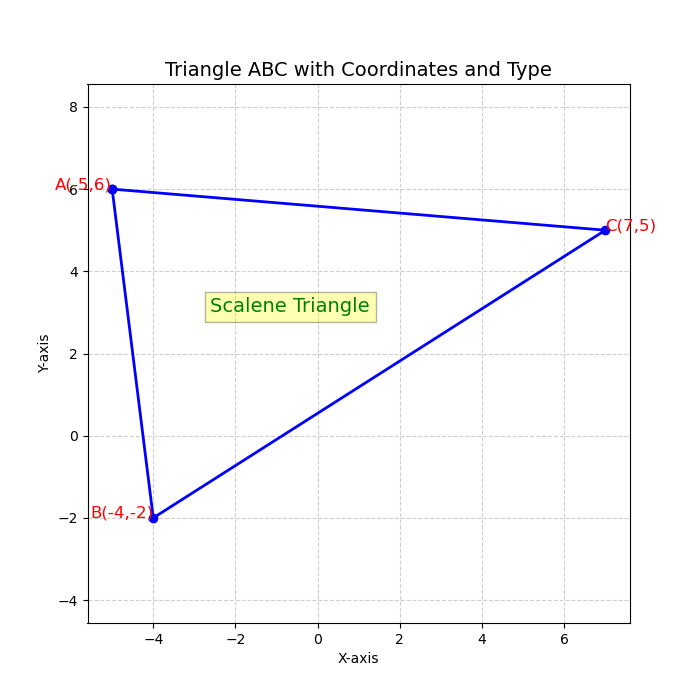
\includegraphics[width=0.7\linewidth]{figs/fig31.png}
       \caption{}
       \label{fig:placeholder}
   \end{figure}

\end{frame}
\begin{frame}{only Python plot}
    

\begin{figure}
    \centering
    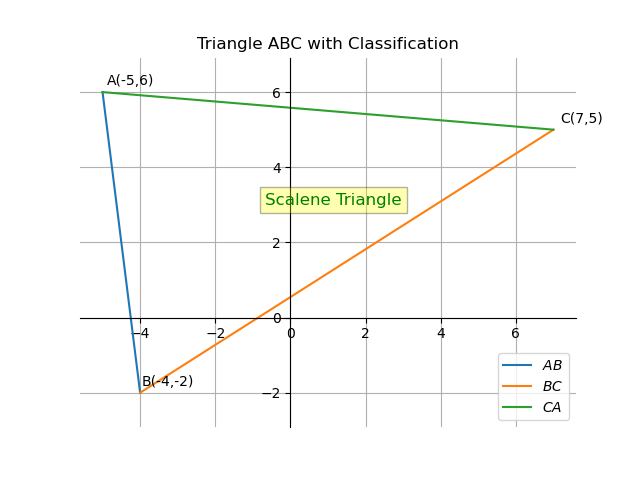
\includegraphics[width=0.9\columnwidth]{figs/Figure32.png}
    \caption{}
    \label{fig:placeholder}
\end{figure}
\end{frame}
\end{document}


